\section{related work}
The section lists the main ideas of the papers the author has read. In order to show the evolution of the technology, those papers are organized in chronological order.
\subsection{Monte Carlo Go paper 1993~\cite{brugmann1993monte, silver2009monte, browne2012survey}}
\subsubsection{Abstract}
This paper present an algorithm for the board game go which attempts to find the best move by simulated 
annealing. Using this method, without including any go knowledge beyond the rules, this paper manages
to a playing strength of about 25 kyu on a $9\times9$ board.
\subsubsection{Introduction}
The author started the discussion using "how would nature play go?" Then the author tried to use simulated 
annealing to solve the problem. The basic idea of the method is simple: 
\begin{inparaenum}
	\item moves are performed randomly with probabilities assigned by the method of simulated annealing;
	\item the value of a position in which the game is over is defined by counting, and 
	\item to find the best move in a given position play the game to the very end as suggested by (i) 
		and then evaluate as in (2); play many such random games, and the best move will be the one which does best on average.
\end{inparaenum}
The author also believes that the idea is simple, and any good idea can be stated simply. In this paper, the authors also tried to convince the readers that this is at least not a bad idea.
\subsubsection{Simulated annealing for mathematical problems}
If you want to find the minimum of one function, if the function is simple enough and depends only on a small number of variables, there are very efficient exact numerical methods to find its local minima. They are all based essentially the same principle. Pick initial values for each variable and compute the function. Change the variables slightly in such a way that the function velue decreases. Repetition allows one to come arbitrarily close to a local minimum. Different algorithms have been invented to optimize the process at each iteration for different classes of functions.

There are several types of problems where there is virtually no alternative to simulated annealing. As it turns out, these exact algorithms are greedy by design, that is given a starting point they greedily walk downhill (following the steepest descent) until they have found a local minimum. But if one is looking for a global minimum among many local ones, and if one does not know before-hand where to look for it, one will never find it.

Two combinatorial optimization, traveling salesman problem. These problems are examples for combinatorial optimization since the configuration space on which function is to be minimized is a discrete, factorially large space. In the traveling salesman problem, there are $N = N \times (N-1) \times \times 1$ possibilities to make an ordered list of N cities.

Second example is to find the arrangement of 25 playing cards in a $5 \times 5$ tableau such that the value of the rows, columns, and diagonals interpreted as hands for poker is maximized.
\subsection{Probabilistic reasoning over time}
In which we try to interpret the present, understand the past, and perhaps predict the future, even when very little is crystal clear.
\subsubsection{Time and uncertainty}
Two cases, car repair, we assume that whatever is broken remains broken during the process of diagnosis; our job is to refer the state of the car from observed evidence.
%\subsubsection{Inference in temporal model}
%\textbf{Filtering:} this is the task of computing the belief state - the posterior distribution ove the most recent state - given all evidence to date. Filtering is also called state estimation. This is what a rational agent does to keep track of the current state so that rational decisions can be made.
%\textbf{prediction:} this is the task of computing the posterior distribution over the future state, given all evidence to date. This is used to calculate the probability distribution of future events.
%\textbf{smoothing:}
%\textbf{Most likely explanation:}
%\subsubsection{SmartGame library}
%The SMARTGAME library contains generally useful game-independent functionality. It includes utility classes, classes that encapsulate non-portable platform-dependent functionality, and classes and functions that help to represent the game state for two-player games on square boards.
\subsection{Fuego software framework~\cite{enzenberger2010fuego}}
FUEGO, as an open source software framework, can facilitate and accelerate research. 
It's able to play the game of Go. The framework supports developing game engines for full-information two-player 
board games, and is used successfully in a substantial number of projects. The FUEGO 
Go program became the first program to win a game against a top professional player in $9 \times 9$ Go.
Advance in theory, such as MCTS and the UCT algorithm have led to breakthrough performance in computer Go.
% This is a paper in 2015 
\subsection{Move evaluation in go using deep convolutional neural networks~\cite{maddison2014move, clark2015training}}
The game of Go is more challenging than other board games, due to difficulty of constructing a position or move evaluation function. This paper investigates whether deep convolutional networks can be used to directly represent and learn this knowledge. The paper trains a 12-layer convolutional neural network by supervised learning from a database of human professional games. The network correctly predicts the expert move in 55\% of positions, equaling the accuracy of a 6 dan human player.

The contributions of thie paper lie in the following aspects. Although CNNs have previously been applied to the game of Go, with modest success, previous architectures have typically been limited to one hidden layer of relatively small size, and have not exploited recent advances in computational power. This paper uses deeper and larger CNNs of 12 hidden layers and several billion connections to represent and learn knowledge. And this increase in depth and size leads to a qualitative jump in performance, suggesting that contrary to previous beliefs, a strong move evaluation function for Go can indeed be represented and learnt by such architectures.

Convolutional neural networks have a long history in the game of Go. Schraudolph Schraudolph
et al. (1994) trained a simple CNN (exploiting rotational, reflectional, and colour inversion symmetries)
to predict final territory, by reinforcement learning from games of self-play. The resulting
program beat a simplistic handcrafted program called Wally. NeuroGo (Enzenberger, 1996) used
a more sophisticated architecture to predict final territory, eyes, and connectivity, again exploiting
symmetries; and used a connectivity pathfinder to propagate information across weakly connected
groups of stones. Enzenberger's program also used reinforcement learning from self-play. When
combined with an alpha-beta search, NeuroGo equalled the performance of GnuGo on 9 $\times$ 9 Go,
and reached around 13 kyu on 19$\times$19 Go. Sutskever \& Nair (2008) applied convolutional networks
to supervised learning of expert moves, but using a small 1 hidden layer CNN; this matched
the state-of-the-art prediction performance, achieving 34.6\% accuracy, but this was not sufficient to
play Go at any reasonable level.

The 12 layer neural network has implicitly understood many sophisticated aspects of Go, including good
shape (patterns that maximise long term effectiveness of stones), Fuseki (opening sequences), Joseki
(corner patterns), Tesuji (tactical patterns), Ko fights (intricate tactical battles involving repeated
recapture of the same stones), territory (ownership of points), and influence (long-term potential
for territory). It is remarkable that a single, unified, straightforward architecture can master these
elements of the game to such a degree, and without any explicit lookahead.

It appears that we now have two core elements that scale effectively with increased computational resources: scalable planning, using Monte-Carlo search; and scalable evaluation functions, using deep neural netowrks. In the future, as parallel computation units such as GPUs continue to increase in performance, we believe that this trajectory of research will lead to considerably stronger programs than are currently possible.

The method might work well, but it also has its own weakness. Notably it sometimes fails to understand the global picture, behaving as if the life and death status of large groups has been incorrectly assessed. Interestingly, it is precisely these global aspects of the game for which Monte-Carlo search excels, suggesting that these two techniques may be largely complementary. We have provided a preliminary proof-of-concept that MCTS and deep neural networks may be combined effectively.
% Facebook paper
\subsection{Better Computer go player with neural network and long-term prediction~\cite{tian2015better, schaeffer2001temporal}}
This work is done by some researchers at Facebook.
\subsubsection{Abstract}
Search is not strictly necessary for machine Go players. A pure pattern-matching approach, based on a deep convolutional neural network that predicts the next move, can perform as well as Monte Carlo Tree Search-based open source Go engine such as Pachi if its search budget is limited.

Darkforest relies on a DCNN designed for long-term predictions. While the previous methods can predict the next move that a human would play 55.2\% of the time. However, whether this accuracy leads to a strong Go AI is not yet well understood. This paper tries to show that DCNN-based move predictions indeed give a strong Go AI, if properly trained.
\subsubsection{Introduction}
Recent study shows that the Go board situation could be deciphered with Deep Convolutional Neural Network. They can predict the next move that a human would play 55.2\% of the time. In this paper, the authors show that DCNN-based move predictions indeed give a strong Go AI, if properly trained. In particular, the authors carefully design the training process and choose to predict next k moves rather than the immediate next move to enrich the gradient signal.
%
%What kind of data is used to train?
%\subsubsection{method}
%\subsubsection{feature channel}
\subsubsection{Network architecture}
This paper uses a 12-layered full convolutional network. Each convolutional layer is followed by a ReLU 
nonlinearity. Except for the first layer, all layers use the same width w = 384. No weight sharing is used. 
We do not use pooling since they negatively affect the performance. Instead of using two softmax outputs to 
predict black and white moves, we only use one softmax layer to predict the next move, reducing the number 
of parameters.
\subsubsection{Long term planning}
Predicting only the immediate next move limits the informaiton received by the lower layers. Instead, we 
predict next k moves from the current board situation. Each move is a separate softmax output. The motivation
is two-fold. First, we want our network to focus on a strategic plan rather than the immediate next move. 
Second, with multiple softmax outputs, we expect to have more supervisions to train the network. 
\subsubsection{Training}
When training, we use 16 CPU threads to prepare the minibatch, each simulating 300 random selected
games from the dataset. In each minibatch, for each thread, randomly select one game out of
300, simulate one step according to the game record, and extract features and next k moves as the
input/output pair in the batch. If the game has ended (or fewer than k moves are left), we randomly
pick one (with replacement) from the training set and continue. The batch size is 256. We use data
augmentation with rotation at 90-degree intervals and horizontal vertical flipping. For each board
situation, data augmentation could generate up to 8 different situations.
Before training, we randomly initialize games into different stages. This ensures that each batch
contains situations corresponding to different stages of games. Without this, the network will quickly
overfit and get trapped into poor local minima.
\subsubsection{Monte carlo tree search}
From the experiments, we clearly show that DCNN is tactically weak due to the lack of search.
Search is a way to explore the solution space conditioned on the current board situation, and build
a non-parametric local model for the game. The local model is more flexible than the global model
learned from massive training data and more adapted to the current situation. The state-of-the-art
approach in computer Go is Monte-Carlo Tree Search (MCTS).
%\subsubsection{Knowledge representation}
%The author tries to give the definition of what knowledge is. Something is strange that this question has never been answered directly. In history, different people have tried to describe it from different prospectives. The authors believe that this question can be answered in terms of five important and distinctly different roles that a representation play.
%\begin{enumerate}
%	\item A knowledge representation is most fundamentally a surrogate, a substitute for the thing itself, used to enable an entity to determine consequences by thinking rather than acting;
%	\item It is a set of ontological commitments;
%	\item It's a fragmentary theory of intelligent reasoning;
%	\item It's a medium for pragmatically efficient computation;
%	\item It's a medium of human expression.
%\end{enumerate}
%Also there are two terminologies, inference, to mean any way to get new expressions from old; give the familiar set of basic representation tools like logic, rule, frames, semantic nets, as knowledge representation technologies.
\subsection{Bayesian Pattern Ranking for Move Prediction in the game of Go~\cite{stern2006bayesian}}
This paper, the authors investigate the problem of learning to predict moves in the board game of Go from game records of expert players. They obtain a probability distribution over legal moves for professional play in a given position.
This distribution can be quite useful, it can serve as a stand-alone player; and it can also be a move selector and move sorter. Two major components: a pattern extraction scheme for efficiently harvesting patterns of given size and shape from expert game; a Bayesian learning algorithm that learns a distribution ove the values of a move given a board position based on hte local pattern context.

Go has emerged as a major challenge for AI with the best computer Go programs currently playing at the level of weak amateur human players. This stands in stark contrast with the state of computer chess where computers play beyond human world class level. In Go, global search is typically replaced with a hybrid of local search, pattern matching and territory estimation.
%\subsubsection{board and pattern representation}
%how to represent a board configuration and the properties of these patterns;
%\subsubsection{local features}
%
%\subsubsection{pattern matching and storing}
%\subsubsection{pattern harvesting}
%\subsubsection{models for move prediction}
%
\subsection{Mimicking Go Experts with Convolutional Neural Networks~\cite{sutskever2008mimicking}}
\subsubsection{The techniques useful for chess are not useful for Go}
First, the nature of the rules of Chess makes it easy to estimate the player with the advantage, simply by counting the pieces. This and similar heuristics allow minimax search to compute a good move reasonably rapidly. In contrast, there is no easy way to determine the player with the advantages in Go. In particular, counting captured pieces does not work for Go because the value of a piece depends more heavily on its surroundings. The ability to raplidly evaluate Go positions prevents minimax searches from finding good moves. Second, typical Chess positions have 40 legal moves, while typical Go positions have 200 legal moves, so the search space is substantially larger. This partly explains why there are still no strong computer Go players.
\subsubsection{Move predictor}
Constructing a fairly accurate move predictor is potentially easier than playing Go well, because an accurate move predictor can occasionally make devastating mistakes which would make it a poor Go player.
\subsection{Mastering the game of Go with deep neural networks and tree search~\cite{silver2016mastering}}
All game of perfect inforamtion has a optimal value function, which determines the outcome of the game. Two factors deterimines the the complexity of the game, braching factor and depth. To improve the performance, the effective search space can be reduced by two general principles. First, the depth of the search may be reduced by position evaluation: truncating the search space at state s and replacing the subtree below s by an approapriate value function that predicts the outcome from state s; Second, the breadth of the search may be reduced by sampling actions from a policy p(a|s) that is a probability distribution over possible moves a in position s. As discussed above, the search space of Go is too large, so it is not possible to traverse the whole space to get the final result. The basic idea is, use the old methods, but combine them. 
\begin{figure*}[!ht]
  \caption{The complexity comparison of different board games}
  \centering
    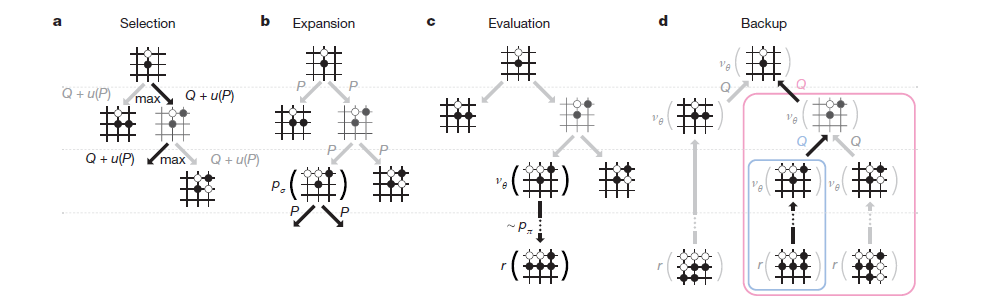
\includegraphics[width=0.9\textwidth]{MCTS-AlphaGo.png}
\end{figure*}
To address this problem, these researchers propose to solve the problem using two parts, policy network and value network. It's trained using supervised learning and reinforcement learning.

The policy network is to imitate the bahaviors of human. Given the current state of the board, the network will return some promising-looking moves. And these information is fed into the value network. The value network will evaluate these moves basically based on the previous games.
\begin{figure*}[!ht]
  \caption{Alpha Go training pipeline.}
  \centering
    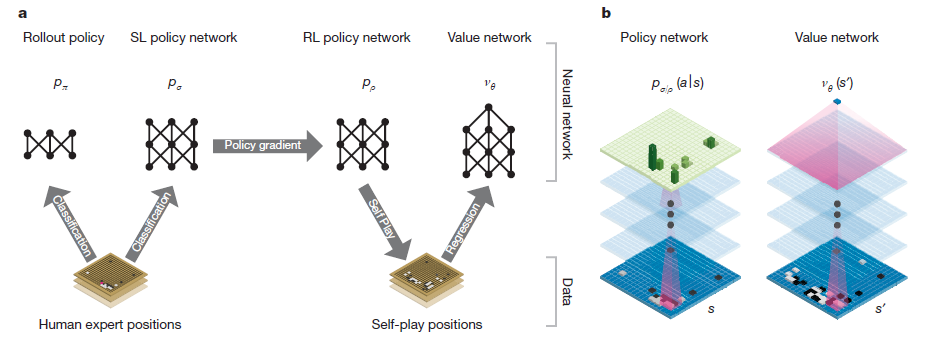
\includegraphics[width=0.9\textwidth]{AlphaGoTrainingPipeline.png}
\end{figure*}
\subsubsection{Supervised learning of policy networks}
This is the first stage of the training pipeline. The training is performed on 30 million positions from the KGS Go Server. The result is a 13 layer policy network
\subsubsection{Reinforcement learning of policy networks}
The second stage of the training pipeline aims at improving the policy network by policy gradient reinforcement learning.
\subsubsection{Reinforcement learning of value networks}
Ideally, we would like to know the optimal value function under perfect play; in practice, we instead estimate the value function for our strongest policy.
\subsubsection{Seaerching with policy and value networks}

\subsubsection{Evaluating the playing strength of AlphaGo}
To evaluate AlphaGo, a single machine version and a distributed version are used:
\begin{inparaenum}
	\item Single machine AlphaGo is many dan ranks stronger than any previous Go program. To provide a greater challenge to AlphaGo, the author also played games with four handicap stones; AlphaGo won 77\%, 86\%, and 99\% of handicap games against Crazy Stone, Zen and Pachi, respectively. The distributed version of AlphaGo was significantly stronger, winning 77\% of games against single-machine AlphaGo and 100\% of its games against other programs;
	\item The distributed version is evaluated against Hui Fan;
\end{inparaenum}
\subsubsection{Discussion}
Deep learning is based on two things: plenty of processing grunt and large amount of data. DeepMind trained its machine on a sample of 30m Go positions culled from online servers where amateurs and professionals gather to play. And by having AlphaGo play against another, slightly tweaked version of itself, more training data can be generated quickly.

How many hardware resources are there? The version playing against Mr Lee uses 1920 standard processor chips and 280 special ones developed originally to produce graphics for video games. At least part of the reason AlphaGo is ahead of the competition is that it runs on more potent hardware.

Go is exemplary in many ways of the difficulties faced by artificial inteligence: a challenge decision-making task, an intractable search space, and an optimal solution so complex it appears infeasible to directly approximate using a policy or value function. The previous major breakthough in computer Go, the introduction of MCTS, led to corresponding advances in many other domains; for example, general game-playing, classical planning, partially observed planning, scheduling, and constraint satisfaction.

Why is it meaningful? The techniques employed in AlphaGo can be used to teach computers to recognize faces, translate between languages, show relevant advertisements to internet users or hunt for subatomic particles in data from atom-smashers. Deep learning is thus a booming business. It powers the increasingly effective image- and voice-recognition abilities of computers, and firms such as Google, Facebook and Baidu are throwing money at it.

In summary, AlphaGo's success can largely be traced to a combination of the following two powerful technologies: 
\begin{inparaenum}
\item Monte Carlo tree search, this involves choosing moves at random and then simulating the game to the very end to find a winning strategy;
\item Deep reinforcement learning, a multi-layered neural network that mimics brain connections, which contains of a "policy network" that selects the next move and a "value network" that predicts the winner of the game. But there is a missing piece, the ability to learn how the world works - such as understanding the laws of physics, and the consequence of one's actions.
\end{inparaenum}
These methods have spanned a long time in the history. They appear in different background. 

%To answer the queation, the more accurate statement is that everyone believed that without some fundamentally new ideas about the structure of Go or its play, computers would never challenge Go masters. People talk about pattern recognition, but never seem to find the right ideas.

As pointed out in this paper~\cite{maddison2014move}, neural network sometimes has its weakness: it sometimes fails to understand the gobal picture, behaving as if the life and death status of large groups would be incorrectly assessed. However, Monte Carlo method can excel in these aspects. If these method were combind, good results are achieved.

